%\begin{comment}
\chapter{Document to Image: Overview of System}
In this project, we trying to generate the keywords from a given news document that is closely match with descriptive metadata of an relevant image.
%\end{comment}


\section{Metadata}
Metadata are defined as the data providing information about one or more aspects of the data, such as:
\begin{enumerate}
\item{Purpose of data}
\item{Date and Time of creation}
\item{Author of data}
\item{Means of creation of data}
\end{enumerate}

A text document's metadata may contain information about how long the document is, who the author is, when the document was written, and a short summary of the document. A digital image may include metadata that describe how large the picture is, the color depth, the image resolution, when the image was created, and other data.

The term `metadata' refers to `data about data'. Widely the term `metadata' is used for two different concepts. 

`Structural metadata' is about the design and specification of data structures and more precisely it should be `data about containers of data'.

`Descriptive metadata', on the other hand is all about the content of data i.e, instance of application data. In our problem, we are trying to utilize the descriptive metadata of images for retrieval. 

\section{Classification of Images}

We tried to classify images annotated to the news articles, based on its relation to the content of the articles. Difficulty level of finding these Images automatically will vary based on its classification.

\subsection*{Representative Images}

Image attached to an article is a representative for the content of documents. and descriptive metadata of image most likely to match the sentence or title from the text. Relatively easy to retrieve image if extracted keywords or phrases.

\begin{comment}
\noindent \cbox{Example-Representative\\}{\textbf{News Text} : Article is about oil spil\\
\textbf{Annotated Image} : Image with description with `oil spil happened in '}
\end{comment}

\begin{center}
    \begin{tabular}{ | p{7.8cm} | p{7.8cm} | }
    \hline
    \textbf{TITLE : }CBI quizzes Amit Shah in Ishrat encounter case & \textbf{METADATA : }CBI has questioned Amit Shah in Ishrat Jahan `fake' encounter case. \\ 
    \hline
    NEW DELHI: Racing to file its supplementary chargesheet in the Ishrat Jahan "fake" encounter case shortly, the CBI on Saturday questioned Amit Shah, a close aide of BJP's prime ministerial candidate, Narendra Modi..... & 
 \raisebox{-\totalheight}{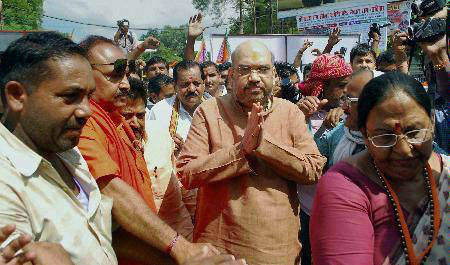
\includegraphics[width=7.8cm]{rep.jpg}}\\
    \hline
\end{tabular}\linebreak
\end{center}

\subsection*{Iconic Images}

Sometimes though articles is not directly talking about the person/entity in the Image, because of it's popularity it is tagged with the article. It is difficult identify exactly same image.\\
\begin{comment}
\noindent \cbox{Example-Iconic Images\\}
{\textbf{News Text} : Wasting Time Is New Divide in Digital Era.\\
\textbf{Image Description} : Facebook Picture.\\
\textbf{News Text} : Any article related to Bollywood news (remake).\\
\textbf{Image Description} : Salman Khan's Image.
}
\end{comment}
\begin{center}
    \begin{tabular}{ | p{7.8cm} | p{7.8cm} | }
    \hline
    \textbf{TITLE : }Is Social Media a Waste of Time? & \textbf{METADATA : }Social Network site : Facebook \\ 
    \hline
    PhDs at billion-dollar research firms are revising their algorithms and texting their marketing departments to counter this argument with new catch-phrases, but it`s all in vain...... & 
 \raisebox{-\totalheight}{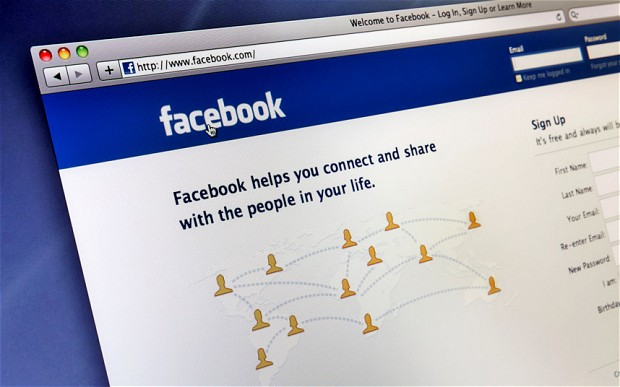
\includegraphics[width=7.8cm]{icon.jpg}}\\
    \hline
\end{tabular}\linebreak
\end{center}


\subsection*{Aspectual Images}
Similar to iconic but image is related to event or aspect described in the article, but article need not necessarily mention the person or entity in image explicitly.

\begin{comment}
\noindent \cbox{Example-Iconic Images\\}{
\textbf{News Text} : Article is about Kolkata Knight riders won trophy \\
\textbf{Image Description} : An image of Mr,Shahrukh Khan holding trophy.\\
\textbf{News Text} : for an article titled `US threatens war while considering talks with Syria, Iran'. \\
\textbf{Image Description} :  Obama's Pictures with Syria map.
}
\end{comment}

\begin{center}
    \begin{tabular}{ | p{7.8cm} | p{7.8cm} | }
    \hline
    \textbf{TITLE : }KKR stunning win over CSK in a pulsating IPL 5 final & \textbf{METADATA : } Shahrukh Khan with IPL 5 Trophy after KKR win 6 \\ 
    \hline
 There was a galaxy of former Indian cricketers in attendance, the brightest lights from Bollywood were in the stands, both teams had some of the biggest stars in the world game but the headlining performance came from little-known...... & 
 \raisebox{-\totalheight}{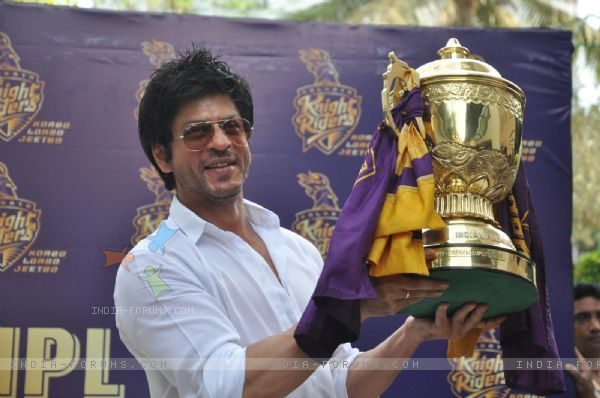
\includegraphics[width=7.8cm]{aspectual.jpg}}\\
    \hline
\end{tabular}\linebreak
\end{center}

\subsection*{Cited Images}
A news provider using an image taken by other providers and citing the source and article with the image. These type of images are rarely seen in the article nowadays.

\subsection*{Historical Images}
Article speaks about event happened at certain time whereas images of past is tagged . This happens majorly due to unavailability images at the time of creating news article.

\noindent \cbox{Example-Historical Images\\}
{\textbf{News Text} : An article is about bomb blast of zaveri bazaar.\\
\textbf{Image Description} : zaveri bazaar before bomb blast.\\
\textbf{News Text} : For an article about Temple's renovation \\ 
\textbf{Image Description} : temple before renovation is being used in the article.}

\subsection*{Partially Relevant Images}
Image attached to news article is relevant to portion of the article but not to the whole article.
\begin{comment}
\noindent \cbox{Example-Partially Relevant Images\\}
{\textbf{News Text} : Oil spillage near Hartlepool causes A19 chaos.\\
\textbf{Image Description} : Drivers faced long delays after a busy dual carriageway was closed for almost two hours due to a two-mile spillage of oil.}\
\end{comment}
\begin{center}
    \begin{tabular}{ | p{7.8cm} | p{7.8cm} | }
    \hline
    \textbf{TITLE : }Oil spillage near Hartlepool causes A19 chaos & \textbf{METADATA : }DRIVERS faced long delays after a busy dual carriageway was closed for almost two hours due to a two-mile spillage of oil. \\ 
    \hline
 A tanker started to leak the fuel on the Norton slip-road onto the A19 northbound at around 1.15pm today (Wednesday). The leak continued as it travelled up the A19 and onto the A689 slip-road, on the outskirts of Hartlepool...... & 
 \raisebox{-\totalheight}{
\includegraphics[width=7.8cm]{partial.jpg}}\\
    \hline
\end{tabular}\linebreak
\end{center}



\section{Overview of System}

\begin{figure}[h]
\begin{center}
\fbox{\scalebox{0.7}{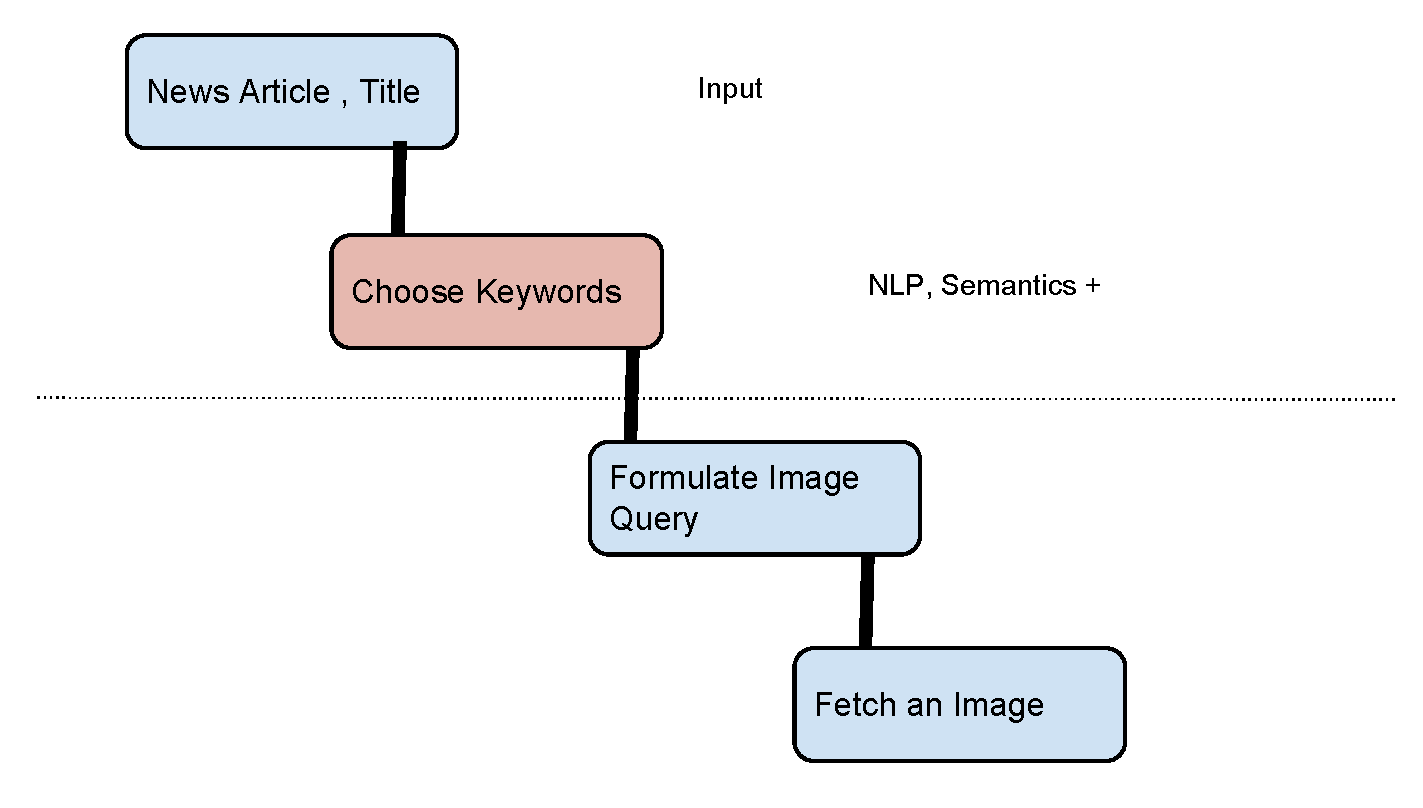
\includegraphics{sys.pdf}}}
\end{center}
\caption{Overall System}
\end{figure}

\noindent \textbf{Input}: Input for the system consist of news article as text document, its title. 

\noindent \textbf{Keyword Extraction}: In this step, top keywords from text document is retrieved. The decision on number of keywords required should be taken here which is difficult to predict.

\noindent \textbf{Formulating Image Search Query}: Image search query needs to formulated based on the keywords extracted. For example, if the keywords are \textit{Sachin}, \textit{WorldCup} then one possible query can be \textit{ Sachin AND Wordcup}. 

\noindent \textbf{Fetching an Image}: Image Query formulated in the previous step must be used for triggering search. An image from result set is used for annotating the news document.


\section{Summary}
In this chapter, we discussed about overall system and classification of images appear in news articles. In the next chapter, we describe the existing works on keyword extraction based supervised and unsupervised approaches.



